\subsection{Geometría del orden}
\setaxsection{B}

El segundo grupo de axiomas establece propiedades de la relación de
\textit{orden}, una relación ternaria entre puntos. Dados tres puntos $A, B, C$
escribiremos $A * B * C$ para indicar que están relacionados mediante la
relación de orden.

Así empieza por tanto la definición de la clase que engloba los axiomas de
orden:

\lstleanfull{order_geometry/basic.lean}{21}{24}

Se puede ver en la línea 22 que esta definición de clase \textit{extiende} la de
la clase \lstinline{incidence_geometry} definida anteriormente. Es decir,
seguimos considerando la relación de incidencia y los axiomas relativos a ella.

Los cuatro \textit{axiomas de orden} son los siguientes:

\begin{ax}\label{ax:B1}
	Si un punto $B$ está entre $A$ y $C$ ($A * B * C$) entonces $A, B, C$ son
	distintos, están en una misma línea y $C * B * A$.
\end{ax}

\lstleanfull{order_geometry/basic.lean}{25}{27}

\begin{ax}\label{ax:B2}
	Para cada dos puntos distintos $A,B$ existe un punto $C$ tal que $A * B * C$.
\end{ax}

\lstleanfull{order_geometry/basic.lean}{28}{28}

\begin{ax}\label{ax:3}
	Dados tres puntos distintos en una línea, uno y sólo uno de ellos está entre
	los otros dos.
\end{ax}

\lstleanfull{order_geometry/basic.lean}{29}{30}

\begin{ax}[Pasch]\label{ax:4}
	Sean $A, B, C$ tres puntos no colineares y $l$ una línea que no contenga a
	ninguno de estos puntos. Si $l$ contiene un punto $D$ que está entre $A$ y $B$
	($A * D * B$) entonces también debe contener un punto entre $A$ y $C$ o un
	punto entre $B$ y $C$.
\end{ax}

\begin{figure}[htbp]
	\centerline{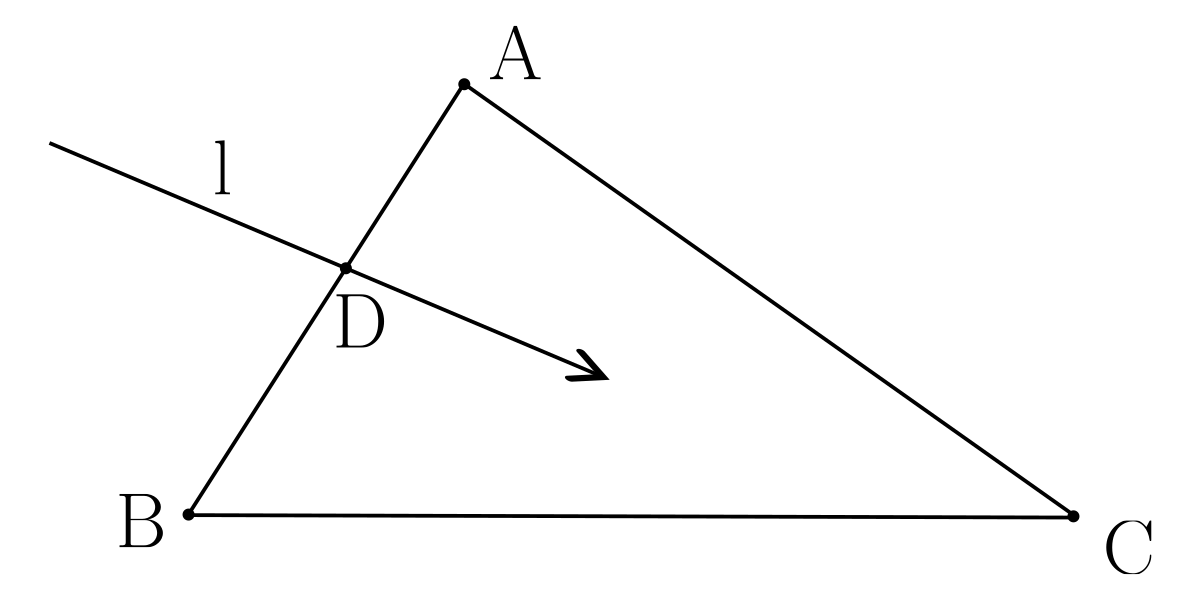
\includegraphics[width=8cm]{./imgs/pasch.png}}
	\label{figure:pasch}
\end{figure}

\lstleanfull{order_geometry/basic.lean}{31}{33}

\subsubsection{Definiciones}\label{ssec:definiciones_orden}

La definición usual de segmentos es la siguiente:

\begin{defin*}[Segmentos]
	Dados dos puntos distintos $A, B$ definimos el \textbf{segmento}
	$\overline{AB}$ como el conjunto de puntos que contiene a $A, B$ y a todos los
	puntos que están entre ellos.
\end{defin*}

Pero en nuestro caso no queremos utilizar teoría de conjuntos y por tanto
queremos evitar nociones como \guillemotleft conjunto de puntos \guillemotright.
Por tanto decimos simplemente que

\begin{defin*}[Segmentos]
	Dos puntos distintos $A, B$ determinan el \textbf{segmento} $\overline{AB}$.
	Diremos que $A$ y $B$ son los \textbf{extremos} del segmento $\overline{AB}$.
\end{defin*}

Esta definición es suficiente para determinar un segmento, pero para establecer
la relación de pertenencia de puntos a segmentos tendremos que complementarla
con otra definición. Para formalizar esta noción utilizamos una estructura:

\lstleanfull{order_geometry/basic.lean}{52}{52}

Cuando se define una estructura en \textit{Lean} se genera de forma automática
un constructor, una función útil para crear términos con tipo la estructura
definida. Dicha función se llamará como la estrucura más la notación
\lstinline{.mk} adjuntada: en este caso se tiene la función
\lstinline{Seg.mk : (neq : A ≠ B) → Seg Point} (observemos cómo los términos
\lstinline{A B : Point} son implícitos en la definición de la estructura).

\begin{defin*}[Pertenencia de puntos a segmentos]
	Decimos que un punto $A$ pertenece a un segmento $\overline{BC}$ si $A$ es
	igual a uno de los extremos del segmento ($B$ o $C$) o está entre ellos
	($B * A * C$).
\end{defin*}

\lstleanfull{order_geometry/basic.lean}{56}{59}

Esta función \lstinline{Seg.in} está dentro del espacio de nombres definido en
la estructura \lstinline{Seg}. Gracias a esto, si tenemos un término de la
estructura \lstinline{seg : Seg Point}, podremos llamar a la función utilizando
la notación de punto \lstinline{seg.in Line P}, en la que el segmento
\lstinline{seg} es pasado como primer argumento a la función \lstinline{seg}.
Por tanto con esta definición y la notación del punto estamos escribiendo la
pertenencia de puntos a segmentos en el orden contrario al usual:
\lstinline{seg.in Line P} significa que el punto \lstinline{P} pertenece al
segmento \lstinline{seg}. Esta notación del punto también permite acceder a los
elementos de una estructura (si consideramos la estructura como un producto
cartesiano de los tipos que la forman, este acceso se puede ver como una
proyección): En la definición de \lstinline{Seg.in} se puede ver como accedemos
a los extremos mediante la notación \lstinline{seg.A}, \lstinline{seg.B}.

Además es importante observar que $A$ pertenece a $\overline{BC}$ si y sólo si
pertenece a $\overline{CB}$, lo que si consideráramos la definición basada en
conjuntos de puntos equivaldría a decir que los segmentos $\overline{BC}$ y
$\overline{BC}$ son iguales. Dicho de otra forma, el orden de los extremos de un
segmento no determina la relación de pertenencia de puntos a dichos segmentos.

\lstleanfull{order_geometry/basic.lean}{73}{77}

Como en el caso de los segmentos, las siguientes definiciones hacen referencia a
nociones propias de la teoría de conjuntos. En nuestra formalización hemos
evitado dichas nociones, por lo que daremos las definiciones adaptadas,
utilizando sólamente los tipos definidos anteriormente.

\begin{defin*}[Triángulos]
	Tres puntos no colineares (por tanto distintos) $A$, $B$ y $C$, determinan
	el \textbf{triángulo} $\triangle ABC$. Los puntos $A$, $B$ y $C$ se llaman
	\textbf{vértices} del triángulo.
\end{defin*}

\lstleanfull{order_geometry/basic.lean}{110}{112}

En este caso también podemos definir funciones mediante la notación de punto que
nos permitan recuperar propiedades sobre una estructura, como por ejemplo la
propiedad de que los vértices del triángulo son distintos:

\lstleanfull{order_geometry/basic.lean}{135}{138}

\begin{defin*}[Pertenencia de puntos a triángulos]
	Decimos que un punto $P$ pertenece al triángulo $\triangle ABC$ si pertenece
	a alguno de los segmentos determinados por sus vértices.
\end{defin*}

\lstleanfull{order_geometry/basic.lean}{142}{146}

Como esta definición se basa en la pertenencia de puntos a segmentos, el orden
en el que consideremos los puntos del triángulo tampoco será determinante para
establecer esta relación de pertenencia.

\begin{defin*}[Rayos]
	Decimos que dos puntos distintos $A, B$ definen el \textbf{rayo}
	$\overrightarrow{AB}$. Dado un rayo $\overrightarrow{AB}$ llamaremos
	\textbf{vértice} del rayo al punto $A$.
\end{defin*}

\lstleanfull{order_geometry/basic.lean}{150}{150}

\begin{defin*}
	Decimos que un punto $P$ \textbf{pertenece} a un rayo $\overrightarrow{AB}$
	si coincide con su vértice $A$ o si $A * B * P$.
\end{defin*}

\lstleanfull{order_geometry/basic.lean}{154}{156}

En este caso el orden de los puntos que determinan un rayo sí que es imporante.
No se tiene como antes que $P$ pertenece a $\overrightarrow{AB}$ si y sólo si
pertenece a $\overrightarrow{BA}$. En términos conjuntistas tendríamos que los
rayos $\overrightarrow{AB}$ y $\overrightarrow{BA}$ son distintos.

\begin{defin*}[Ángulos]
	Dos rayos $\overrightarrow{AB}$ y $\overrightarrow{AC}$ con el mismo vértice
	y tales que $A$, $B$ y $C$ no están alineados determinan un ángulo.
	El vértice de los rayos que determinan el ángulo se llama \textbf{vértice}
	del ángulo. Denotaremos dicho ángulo por $\angle ABC$.
\end{defin*}

\lstleanfull{order_geometry/basic.lean}{160}{163}

Como en la definición de ángulo estamos considerando dos rayos con un punto en
común, se puede observar que tres puntos no alineados determinan un ángulo.
Podemos definir de esta manera un otro constructor para ángulos:

\lstleanfull{order_geometry/basic.lean}{184}{192}

Observemos que en esta definición hemos utilizado el modo táctico en una
definición, lo cual es un recurso útil para construir términos complejos.

\begin{defin*}
	Decimos que dos puntos \textbf{están del mismo lado del plano} respecto de una
	recta si el segmento que los une no contiene ningún punto de la recta.
\end{defin*}

\lstleanfull{order_geometry/basic.lean}{198}{199}

\begin{defin*}[Lados de una línea]
	Decimos que dos puntos están del mismo \textbf{lado de una línea} respecto
	de un punto si los tres puntos están alineados y el segmento que los une no
	contiene a dicho punto.
\end{defin*}

\lstleanfull{order_geometry/basic.lean}{226}{228}

\subsubsection{Resultados}%

Los teoremas que se pueden deducir de este segundo grupo de axiomas son
considerablemente más complicados de demostrar que los del primer grupo. En
particular son demostraciones que tienen detalles técnicos difíciles de
formalizar. \textit{Meikle} y \textit{Fleuriot} han
formalizado~\cite{meikleFormalizingHilbertGrundlagen2003} resultados de esta
sección utilizando el asistente de demostración \textit{Isabelle/Isar}. En el
artículo exponen que la demostración del \textit{Teorema 3} del libro de
Hilbert~\cite{hilbertFoundationsGeometry} incluye pasos que se apoyan en
intuiciones proporcionadas por un dibujo y no están completamente justificados
desde el punto de vista lógico formal.

El teorema tiene el siguiente enunciado:

\setcounter{tma}{2}
\begin{tma}
	Dados dos puntos distintos $A$ y $C$ existe un tercer punto $B$ que se
	encuentra entre ellos: $A * B * C$.
\end{tma}

Y esta es su formalización en \textit{Lean}.

\lstleanfull{order_geometry/propositions.lean}{17}{17}

Debido a la complejidad de la demostración, explicada en detalle en el
artículo~\cite{meikleFormalizingHilbertGrundlagen2003}, y a la falta de tiempo,
no hemos formalizado la demostración de este resultado. Pero nos ha resultado
particularmente interesante la lectura de este trabajo, que nos ha descubierto
una aplicación más de la formalización asistida por computadores: estos métodos
formales permiten estudiar resultados publicados en todo su detalle,
no sólo verificando su corrección sino además aportando información sobre la
forma de trabajar y pensar de grandes matemáticos como Hilbert. Citando al
artículo:

\begin{displayquote}
	Es interesante señalar que la suposición predominante en matemáticas es que
	las demostraciones de Hilbert parecen menos intuitivas, pero tienen un rigor
	aumentado. La prueba Isar muestra que el trabajo de Hilbert puede hacerse
	aún más riguroso con la ayuda de máquinas. Hilbert claramente utilizó un
	diagrama para ayudar a la intuición geométrica y hacer muchas suposiciones.
	Esto parece estar en desacuerdo con su afirmación de que no se necesitaba
	intuición geométrica para derivar los teoremas presentados en el Grundlagen.
\end{displayquote}

El resultado de esta sección que sí hemos formalizado se refiere a la relación
de \textit{estar del mismo lado del plano respecto de una línea}.

\begin{prop}
	La relación de estar del mismo lado del plano respecto de una línea es una
	relación de equivalencia.
\end{prop}

La librería \textit{mathlib} contiene definiciones sobre relaciones de
equivalencia que podemos utilizar: las definiciónes de reflexividad, simetría y
transitividad. Por tanto se tienen tres resultados referentes a estas tres
propiedades. Hemos incluido las demostraciones de las dos primeras propiedades,
pero debido a su extensión no la de la transitividad, que se puede consultar en
el repositorio.
\todo{citar repositorio o anexo}
\todo{¿Está terminada la demo de la transitividad?}

\lstleanfull{order_geometry/propositions.lean}{25}{31}
\lstleanfull{order_geometry/propositions.lean}{34}{50}
\lstleanfull{order_geometry/propositions.lean}{59}{61}

Con esto, en \textit{mathlib}, las relaciones de equivalencia se definen como
estructuras que contienen las demostraciones de estas tres propiedades:

\lstleanfull{order_geometry/propositions.lean}{201}{205}





